\section{标准模型}

正如上文提到的那样,标准模型是现在最为广泛接受的描述电、弱、强三种相互作用的理论。像门捷列夫的元素周期表一样,标准模型也成功的预言了许多粒子和现象,并且得到了实验的证实。标准模型中,基本粒子由轻子、夸克、规范矢量玻色子以及Higgs玻色子构成。如图 \ref{fig:ParticleTable} 所示
\begin{figure}[htb]
    \begin{center}
    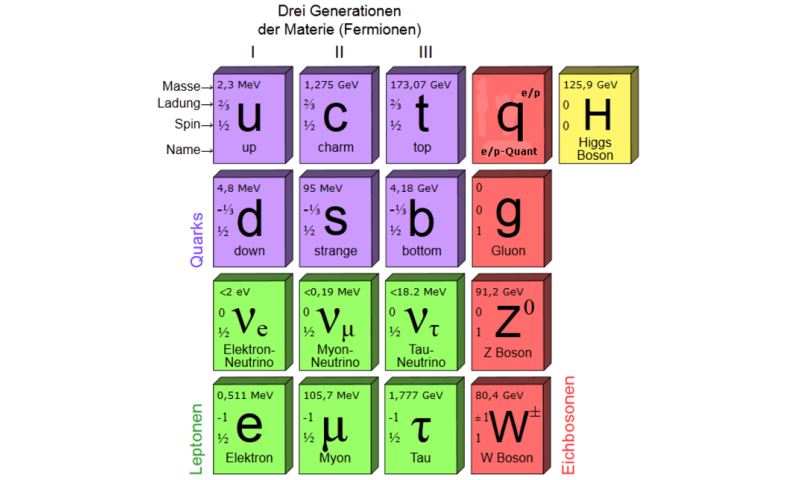
\includegraphics[width=\textwidth,clip]{figures/Chapter1/ParticleTable.png}
    \end{center}
    \caption[标准模型中的基本粒子]{标准模型中的基本粒子}
    \label{fig:ParticleTable}
\end{figure}
其中轻子和夸克为自旋为1/2的费米子,每一种轻子和夸克都有其对应的反粒子。轻子共分为三代(Generation),电子、缪子(muon)、tau轻子和其对应的中微子分别组成不同的代。每一代轻子和其反粒子都带有被称为轻子数的量子数,轻子严格地遵守轻子数守恒定律。夸克和轻子之间存在着某种对称性,自然,夸克也存在和轻子类似的代的概念,被分为三代夸克,如图 \ref{fig:ParticleTable}所示。除了自旋为1/2的费米子以外,标准模型中还存在着四种规范矢量玻色子作为费米子之间的相互作用的传播子存在。其中光子,$W^{\pm}$以及 $Z^0$玻色子为自旋为1的粒子,而Higgs玻色子为目前唯一自旋为0的玻色子。他的引入源于解决弱相互作用的对称性破缺问题时引入的Higgs场,当粒子与Higgs场相互作用的时候其不再以光速进行传播并且获得质量。而那些不与Higgs场有相互作用的粒子,例如光子、胶子等则保持质量为零。

在量子力学建立之初,人们只是用它来处理粒子这种物质的存在,而对于物理学中另一个很重要的概念——场却没有进行量子化的处理,仍是经典的,并没有将其和粒子放在同等地位。这就导致有一些问题仍然无法得到很好的解决,例如光电效应、原子发射和吸收光子以及粒子的产生和湮灭等问题。这就让人们开始考虑将量子化的概念从单粒子拓展到场的范围。人们开始尝试把克莱因-高登和狄拉克方程解释成为场方程,即将其中的波函数解释为经典场,从而开始了场的量子化过程。在历史上人们首先对电磁场进行了量子化。得到了处理电磁场相互作用的理论,被称为量子电动力学(Quantum Electrodynamics, QED)。电磁相互作用的传播子为光子。

之后在处理中子的$\beta$衰变的时候,费米意识到电磁相互作用不可能产生这个过程,应该是由于某种新的相互作用而引起了中子的$\beta$衰变过程。这种新的相互作用就是弱相互作用\cite{Fermi:1934n j j j j j j}。弱相互作用的强度远弱与电磁相互作用,比电磁相互作用弱了大约$10^{11}$倍。其传播子为$W^{\pm}$以及 $Z^0$。

1937年,汤川秀树类比于描写电磁相互作用的QED理论,提出核力是通过中子和质子之间的一种具有质量的基本粒子来传递的。基于此,汤川预言有一种新的粒子存在,其质量应该介于电子和质子之间,汤川将这种新粒子称为介子(Meson)。后来,汤川预言的这种粒子于1947年被发现,被称为$\pi$介子。至此,粒子世界的主要角色似乎已经齐全了。但在同一年,随着奇异粒子的发现,这种“齐全”的错觉被无情地打破,人们意识到现有的理论不足以解释越来越多的被发现的新粒子。这样人们就有了一个很自然的疑问:这些新粒子是否还有着自己的内部结构?

之后夸克模型便被提出用以解释强子的结构问题。1964年由默里·盖尔曼和乔治·茨威格分别独立提出了夸克模型。其认为强子由三种基本的构造单元组成,这三种不同的构造单元被称为具有三种不同味(Flavor)的夸克(Quark),分别是上夸克(up)、下夸克(down)和奇异(strange)夸克。夸克模型很好地解释了强子的生成和湮灭问题,但在处理一些粒子的组分的时候遇到了困难。按照夸克模型,$\Omega^-$应该有三个s夸克组成且都处于轨道运动的基态,又因为$\Omega^-$的总自旋角动量为$\frac{3}{2}\hbar$,这就要求每一个s夸克的自旋都应该是$\frac{1}{2}\hbar$,明显地违背了泡利不相容原理。基于这个事实,人们开始猜测是否还有一种新的未知的量子数。1965年南部阳一郎研究了这个问题并提出夸克应该有一种新的量子数,他称之为色(Color),从此量子色动力学(Quantum Chremodynamics, QCD)走上了粒子物理学的舞台。

